Motion is a simple concept representing playback state (media clock), as well
as functions for accessing and manipulating this state (media controls). As
such, similar constructs are found in most multimedia frameworks.

\begin{figure}[h]
%\sidecaption
\centering
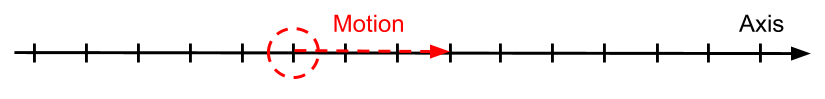
\includegraphics[scale=.4]{fig/motion-axis.png}
\caption{Motion: point moving along an axis. The current position
is marked with a red circle (dashed), and forward velocity of 3 units per second is
indicated by the red arrow (dashed).}
\label{fig:motion}
\end{figure}

As illustrated in Fig.~\ref{fig:motion}, motion represents movement (in real-time)
of a point, along an axis (timeline). At any moment the point has well
defined position, velocity and acceleration\footnote{Some animation frameworks
support acceleration. Acceleration broadens the utility of motions, yet will
likely be ignored in common use cases in classical media (see
Sect.~\ref{sec:toomuch}).}. Velocity and acceleration describe continuous
movements. Velocity is defined as position-change per second, whereas
acceleration is defined as position- change per second squared. Discrete jumps
on the timeline are also supported, simply by modifying the position of the
motion. A discrete jump from position A to C implies that the transition took
no time, and that no position B (between A and C) was visited. Not moving
(i.e. zero velocity and acceleration) is a special case of movement.

\runinhead{Internal State.}
\label{sec:internalstate}
Motion is defined by an internal clock and a vector (position, velocity,
acceleration, timestamp). The vector describes the initial state of the
current movement, timestamped relative to the internal clock. This way, future
states of the motion may be calculated precisely from the initial vector and
elapsed time. Furthermore, application programmers may control the motion
simply by supplying a new initial vector. The motion concept was first
published under the name Media State Vector (MSV)~\cite{msv}.


\subsection{Timing object API}
\label{sec:motionapi}

Timing objects provide access to motions. Timing objects may be constructed
with a URL to an online motion. If the URL is omitted, it will represent a
local motion instead.

\begin{lstlisting}[caption=Constructing a timing object.]
var URL = "...";
var timingObject = new TimingObject(URL);
\end{lstlisting}

The \emph{Timing object API} defines two operations, \emph{query} and
\emph{update}, and emits a \emph{change} event as well as a periodic
\emph{timeupdate} event.


\runinhead{query():} 

The query operation returns a vector representing the current state of the
motion. This vector includes position, velocity and acceleration, as well as a
timestamp. For instance, if a query returns position 4.0 and velocity 1.0 and no acceleration, a
new query one second later will return position 5.0.

\begin{lstlisting}[caption=Querying the timing object to get a snapshot vector.]
var v = timingObject.query();
console.log("pos:" + v.position);
console.log("vel:" + v.velocity);
console.log("acc:" + v.acceleration);
\end{lstlisting}


\runinhead{update(vector):} 

The update operation accepts a vector parameter specifying new values for
position, velocity and acceleration. This initiates a new movement for the
motion. Omitting say position implies that the current position will be used.
So, an update with velocity 0 pauses the motion at the current position.

\begin{lstlisting}[caption=Updating the timing object.]
// play, resume
timingObject.update({ velocity: 1.0 }); 
// pause
timingObject.update({ velocity: 0.0 });
// jump and play from 10
timingObject.update({ position: 10.0, velocity: 1.0});
// jump to position 10, keeping the current velocity
timingObject.update({ position: 10.0 });
\end{lstlisting}


\runinhead{timeupdate event:}

For compatibility with existing HTML5 media elements and an easy way to update graphical elements, a \emph{timeupdate} evens is emitted periodically.

\runinhead{change event:}

Whenever a motion is updated, event listeners on the timing object (i.e. media components)
will immediately be invoked. Note that the \emph{change} event is not emitted
periodically like the \emph{timeupdate} event of HTML5 media elements. The change event signifies the start of a
new movement, not the continuation of a movement.



\begin{lstlisting}[caption=Monitoring changes to the motion through the change event.]
timingObject.on("change", function (e) {
  var v = motion.query();
  if (v.velocity === 0.0 && v.acceleration === 0.0) {
    console.log("I'm not moving!");
  } else {
    console.log("I'm moving!");
  }
});
\end{lstlisting}




\subsection{Programming with motions}


\runinhead{Using motions:}

Motions are resources used by Web applications, and the developer may define
as many as required. What purposes they serve in the application is up to the
programmer. If the motion should represent media offset in milliseconds, just
set the velocity to 1000 (advances the position of the motion by 1000
milliseconds per second). Or, for certain musical applications it may be
practical to let the motion represent beats per second.

\runinhead{Timing converters:}

A common challenge in media synchronization is that different sources of media
content may reference different timelines. For instance, one media stream may
have a logical timeline starting with 0, whereas another is timestamped with
epoch values. If the relation between these timelines is known (i.e.
\emph{relative skew}), it may be practical to create a skewed timing object
for one of the media components, connected to the motion. This is supported by
\emph{timing converters}. Multiple timing converters may be connected to a
motion, each implementing different transformations such as scaling and
looping. Timing converters may also be chained. Timing converters implement
the \emph{timing object API}, so media components can not distinguish between
a timing object and a timig converter. A number of timing converters are
implemented in the Timingsrc programming model~\cite{timingsrc}.

\runinhead{Flexibility:}
\label{sec:toomuch}

The mathematical nature of the motion concept makes it flexible, yet for a
particular media component some of this flexibility may be unnecessary, or
even unwanted. For instance, the HTML5 media player will typically not be able
to operate well with negative velocities, very high velocities, or with
acceleration. Fortunately, it does not have to. Instead, the media player may
define alternative modes of operation as long as the motion is in an
unsupported state. It could show a still image every second for high velocity,
or simply stop operation altogether (e.g. black screen with error message).
Later, when motion re-enters a supported state, normal operation may be
resumed for the media player.


\subsection{Online Motion}
\label{sec:motionsync}

The timing object API is particularly designed to mediate access to online motions,
as illustrated by Fig.~\ref{fig:model-repeat}. \emph{Update} operations are forwarded to the
online motion, and will not take effect until notification is received from
the online motion and \emph{change events} are emitted. In contrast, \emph{query} is a local
(and cheap) operation. This ensures that media components may sample the
motion frequently if needed. So, through the Timing Object API, online motions
are made available to Web developers as local objects. Only the latency of the
update operation should be evidence of a distributed nature.

\begin{figure}[h]
%\sidecaption
\centering
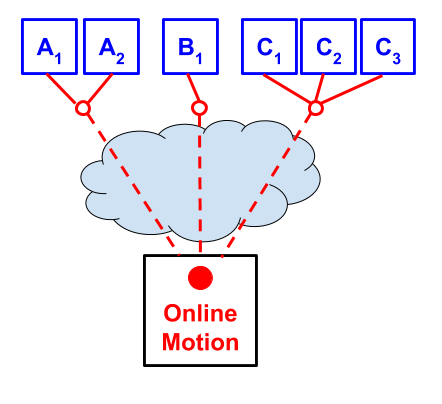
\includegraphics[scale=.3]{fig/motion-model-2.png}
\caption{Timing objects (red unfilled circles) mediate access to online motion. Timing objects may be shared by independent mediacomponents within the same browsing context.}
\label{fig:model-repeat}
\end{figure}

To support this abstraction, precise, distributed \emph{motion
synchronization} is required. In particular, the internal \emph{clock} of the
motion must be precisely synchronized with the clock at the online motion
server. Synchronized system clocks (e.g. NTP~\cite{ntp} or PTP~\cite{ptp}) is
generally not a valid assumption in the Web domain.  As a consequence, an
alternative method of estimating a shared clock needs to be used, for example
by sampling an online clock directly. In addition, low latency is important
for user experiences. Web agents should be able to join synchronization
quickly on page load or after page reload. To achieve this, joining agents
must quickly obtain the current vector and the synchronized clock. For some
applications the user experience might also benefit from motion updates being
disseminated quickly to all agents. Web agents should also be able to join and
leave synchronization at any time, or fail, without affecting the
synchronization of other agents. Motion synchronization is discussed in more
detail in~\cite{msv}.

\emph{InMotion} is a hosting service for online motions, built by spin off
company Motion Corporation~\cite{mcorp}. A dedicated onlice service supporting
online motions is likely key to achieving non-functional goals, such as
high availability, reliability and scalability. Evaluation of
motion synchronization is presented in Sect.~\ref{sec:eval}.

Finally, the timing object API emphasizes an attractive programming model for
multi-device media applications. In particular, by making online motions
available under the same API as local motions (see Sect.~\ref{sec:motionapi}),
media components may be used in single-page as well as multi-device media
experiences, without modification. Also, by hiding the complexity of
distributed motion synchronization, application developers may focus on
building great media components using the timing object API. As such, the
timing object API provides much needed separation of concern in multi-device
media.

\subsection{Synchronizing Audio and Video}
\label{sec:avsync}

On the Web, playback of audio and video is supported by HTML5 media
elements\cite{html5media}. Synchronizing media elements relative to a timing
object means that the \emph{currentTime} property (i.e. media offset) must be
kept equal to the position of the timing object at all times, at least to a
good approximation. The general approach is simply to monitor the media
element continuously, and try to rectify whenever the synchronization error
grows beyond a certain threshold. For larger errors \emph{seekTo} is used. This is
typically the case on \emph{page load}, or after timing object \emph{change} events. Smaller
errors are rectified gradually by manipulating \emph{playbackrate}. \emph{SeekTo} is
quite disruptive to the user experience, so support for variable playbackrate
is currently required for high quality synchronization.

\emph{MediaSync} is a JavaScript library allowing HTML5 media elements to be
synchronized by timing objects. The MediaSync library targets usage across the
most common Web browsers, so it is not optimized for any particular scenario.
Though synchronization of HTML5 media is simple in theory, it involves a few
practical challenges, as indicated in Sect.~\ref{sec:web-html}. First,
\emph{currentTime} is only a coarse representation of the media offset, and it
fluctuates considerably when compared to the system clock. The MediaSync
library solves this by collecting a backlog of samples, from which a value of
currentTime can be estimated. Building up this backlog requires some samples,
so it may take more than a second for estimates to stabilize. Another issue
relates to unpredictable time-consumption in media control operations. In
particular, seekTo(X) will change currentTime to X, but it will require a non-negligible 
amount of time to do so. In the context of synchronization, it aims
for a fixed target when it should be aiming for a moving target. The MediaSync
library compensates for this by overshooting the target. Furthermore, in order
to overshoot by the correct amount, the algorithm collects statistics from
every seekTo operation. Surprisingly perhaps, this strategy works reasonably
well. Evaluation for the MediaSync library is presented in Sect.~\ref{sec:eval}.


\subsection{Synchronizing timed data}
\label{sec:sequencer}

Synchronization of timed data using timing objects is an important challenge.
Timed data such as subtitles, tracks, scripts, logs or time series typically
include items tied to \emph{points} or \emph{intervals} on the timeline.
Synchronization then involves activating and deactivating such items at the
correct time, in reference to a timing object. To simplify programming of
media components based on timed data, a generic \emph{Sequencer} is defined.
The sequencer is similar to the HTML5 track element~\cite{html5track}, but is
directed by the timing object instead of a HTML5 media
element~\cite{html5media}. Web developers register cues associated with
intervals on the timeline, and receive event upcalls whenever a cue is
activated or deactivated. The sequencer fully supports the timing object,
including skipping, reverse playback and acceleration. It may be used for any
data type and supports dynamic changes to cues during playback.

\begin{figure}[h]
%\sidecaption
\centering
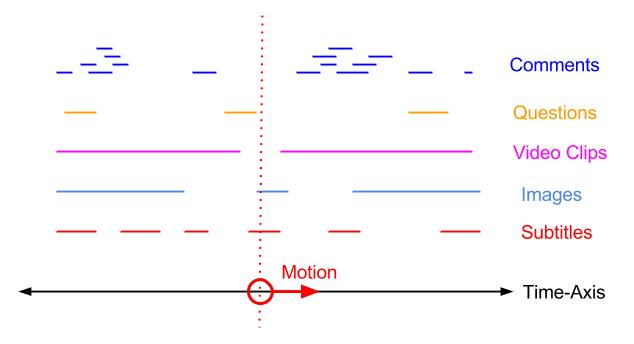
\includegraphics[scale=.4]{fig/sequencer.jpg}
\caption{Five data sources of timed data, with items tied to intervals on the timeline. Motion along the same timeline defines which items are active (vertical dotted line), and precisely when items will be activated or deactivated.}
\label{fig:sequencer}
\end{figure}


The sequencer is implemented as a JavaScript library and made available as
part of the open-source \emph{Timingsrc}~\cite{timingsrc} programming model
(see Sect.~\ref{sec:standard}). In the interest of precisely synchronized
activation and deactivation and low cpu consumption, the sequencer
implementation is not based on frequent polling. Instead, the deterministic
nature of the timing object allows events to be calculated and scheduled using
\emph{setTimeout}, the timeout mechanism available in Web browsers. Though
this mechanism is not optimized for precision, Web browsers may be precise
down to a few milliseconds. The sequencer is presentation in further detail in~\cite{sequencer}.






